\documentclass[a4paper, 10pt]{report}

\usepackage[T1]{fontenc}
\usepackage[utf8]{inputenc}
\usepackage[french]{babel}
\usepackage{tcolorbox}

\usepackage[top=20mm, bottom=20mm, left=10mm, right=10mm]{geometry}

\usepackage{hyperref}

\usepackage{mathpazo}
\usepackage{xcolor}
\definecolor{raspberry}{rgb}{0.737,0.067,0.259}

\usepackage{fancyhdr}
\pagestyle{fancy}

\usepackage[ddmmyyyy]{datetime}
\renewcommand{\dateseparator}{/}

\usepackage{listings}
\usepackage{tcolorbox}
\tcbuselibrary{listings}

\newtcblisting{commandshell}{
	colback=black,
	colupper=white,
	colframe=orange!75!white,
	listing only,
	listing options={style=tcblatex,language=sh},
	every listing line={
		\textcolor{green}{\small\ttfamily\bfseries pi@raspberrypi}:\textcolor{blue}{\small\ttfamily\bfseries \~\ \$\ }
	}
}

\fancyhead[L]{Version du 22/10/2020,\\ modifié le \today}
\fancyhead[C]{\textit{Setup du Buggy du Hardware à la configuration}}
\fancyhead[R]{Swarm Drone Flight}
\fancyfoot[L]{Tristan DRUSSEL}
\fancyfoot[R]{\jobname.pdf}
\headheight = 15pt

\begin{document}

\begin{center}
\LARGE{\textbf{Setup du Buggy du Hardware à la configuration}}
\end{center}

\chapter{Board de composant}
%INTRODUCTION
Afin de supporter tous les composants de notre projet, 
nous avons décider de réaliser une plaque à fixer sur le buggy.
Sur cette plaque, il y aura des trous afin de fixer une majorité de composant.


\section{Composants présents}

Nous avons pensé dans un premier temps à fixer les composants suivant sur la board:
\begin{enumerate}
\item Raspberry Pi ou Jetson Nano
\item Pixhawk
\item Module RTK Rover
\item LIDAR
\item GPS 
\item Télémétrie(s)
\item Buzzer
\item Bouton
\item Carte d'alimentation
\item Receveur RC et Sérialiseur
\end{enumerate}
Dans un second temps, nous pensons aux passages et à la fixation des câbles sur la board.
\section{Réalisation}
Nous avons réalisé cette planche avec le logiciel de CAO open source, \href{freecad.org}{FreeCAD}. Une fois le plan 2D réalisé nous pouvons passer en 3D et inclure les différents composant afin de vérifier si tout s'agençait correctement.
\begin{figure}[!h]
\includegraphics[scale=0.5]{fig/vue1.png}
\end{figure}
\newpage

\section{Plan}

Voici donc un plan de la board, avec les emplacements de chaque composant.
\begin{figure}[!h]
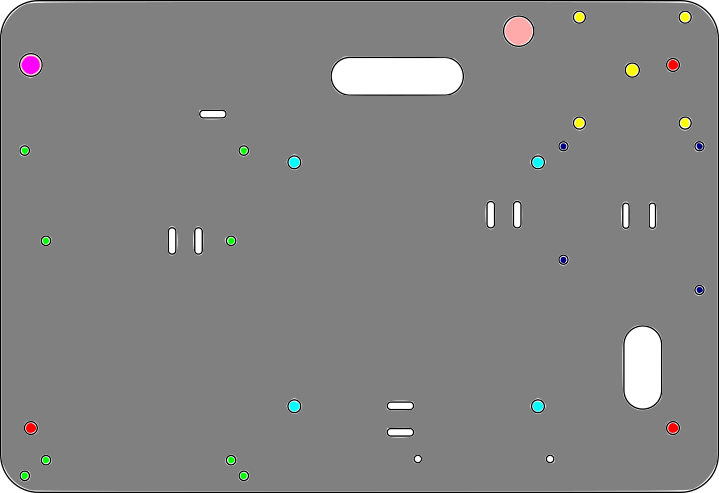
\includegraphics[scale=0.5]{fig/plan.png}
\end{figure}
\begin{enumerate}
\item En Rouge: la fixations au chassis prévus pour des entretoises M3
\item En Cyan: la fixation du Pixhawk sur platine normalisée 65*65 avec entretoise M3, il s'agit aussi de la position pour un LIDAR ou un Module RTK
\item En Vert: les fixations d'une RaspberryPi ou d'une Jetson Nano avec des vis M2
\item En Jaune: la fixation du GPS
\item En Bleu: la fixation de la carte d'alimentation et du sérialiseur avec des vis M2
\item En Rose: la fixation d'une antenne de télémétrie pour XBee
\item En Rose pâle: la fixation d'un buzzer de 30mm
\end{enumerate}

\chapter{Branchement}
	Dans la configuration par défaut
\chapter{Configuration}
\subsection{Télémétrie}
\subsubsection{Antennes de télémétrie}
Les antennes de télémétrie sont des antennes permettant la communication point par point.
Elles sont connectés avec une nappe de 6 fils sur la Pixhawk sur les ports \texttt{TELEM X}.
Elles peuvent aussi se connecter en USB sur un ordinateur pour les configurer ou servir de \textit{Ground Control Station}.

 Elle fonctionne par paire et doivent partager le même identifiant de réseau.
 
\paragraph{Configuration}
Les antennes de télémétrie sont \texttt{Plug and Play}. Si il n'y a que deux antennes, la liaison s'effectue sans soucis. En cas de doute, vous pouvez toujours reflasher le même firmware sur les deux antennes.
\begin{itemize}
	\item Mission Planner: Onglet Configuration=>Optionnal Hardware=>SiK Radio: Upload Firmware
	\item QGround Control: Onglet Setup=>Firmware: débrancher et rebrancher votre antenne pour démarrer l'upload
\end{itemize}
\paragraph{Identifiant de réseau} L'identifiant de réseau est par défaut 25. Si plusieurs drones fonctionnement dans la même zone, il faut penser à changer cette identifiant de réseau. Comment faire:
\begin{itemize}
	\item Mission Planner: Onglet Configuration=>Optionnal Hardware=>SiK Radio: NetID
	\item QGround Control: \texttt{XXXXXX}
\end{itemize}


\begin{tcolorbox}[center,width=0.9\textwidth, colframe=red!90!orange, colback=orange!25, arc=3mm,boxrule=1mm, sharp corners=east,title=En cas de problème]
			Si les deux antennes clignotent vert, elles ne sont pas connectées entre elle. Cela peut venir des points suivants:
			\begin{itemize}
				\item les deux antennes n'ont pas la même version du Firmware.
				\item les deux antennes n'ont pas le même NetID.
				\item si ce n'est pas cela tenter de restaurer la configuration par défaut.
			\end{itemize}
			Les deux antennes sont liés mais ne communiquent pas:
			\begin{itemize}
				\item Le baudrate n'est pas bien saisi.
				\item ...
			\end{itemize}
 \end{tcolorbox}
\subsubsection{Réseau de XBee}
Les modules XBee sont des modules de communication fonctionnement de plusieurs manières commercialisés par la marque Digi mais plusieurs alternatives existent. Leur mode de fonctionnement sont multiple mais le point qui nous intéresse ici, c'est leur fonctionnalité \texttt{Digi-Mesh}. Cette fonctionnalité permet de réaliser un réseau où chaque module à un rôle et permet une communication simple.
\paragraph{Configuration}
Afin de pouvoir faire fonctionner les modules XBee en réseau avec un Pixhawk par exemple, il faut changer quelques paramètres. Pour cela, il y a plusieurs options, envoyer des commandes AT à partir d'un terminal série ou passer par le logiciel de Digi \texttt{XCTU}. Ce logiciel permet d'effectuer des opérations simples sur les XBee.
\paragraph{Identifiant du réseau}
Les XBee fonctionnent sur un réseau, tous les modules doivent partager le même comme avec les antennes de télémétrie. Laisser l'identifiant par défaut peut poser des problèmes si d'autres personnes utilise des modules XBee à porter d'un de vos modules.
\subparagraph{Identifiant de la node}
Afin de pouvoir simplifier la reconnaissance de son réseau, il peut être important de nommer chaque node de son réseau et pouvoir ainsi effectuer un suivi des modules fonctionnels.
\paragraph{Baudrate}
Le baudrate est la vitesse de communication de la liaison UART. Par défaut celle ci est configurée à 9600baud mais le Pixhawk fonctionne à une vitesse de 57600baud pour les communications télémétriques. Il faut donc régler tous les modules à 57600baud.
\paragraph{Rôle dans le réseau}

\paragraph{Connection sur QGroundControl ou MissionPlanner}


\section{Fonctionnement}
\chapter{Pour aller plus loin}
\section{DroneKit}
\section{Paramètre de Ardupilot}
	Extrait de la liste disponible ici: https://ardupilot.org/rover/docs/parameters.html
	\subsection{Configuration}
		\paragraph*{\texttt{SYSID\_THISMAV}}  Identifiant MAVLINK du drone
		\paragraph*{\texttt{SYSID\_MYGCS}}  Identifiant MAVLINK de la station MAVLINK qui lui parle.
		\paragraph*{\texttt{LOG\_BITMASK}} Changement des paramètres de log.
		\paragraph*{\texttt{CRUISE\_SPEED}} Vitesse de croisière en m/s pour le mode AUTO/GUIDED
		\paragraph*{\texttt{CRUISE\_THROTTLE}} Commande de puissance au démarrage en %
		\paragraph*{\texttt{FS\_CRASH\_CHECK}} Que faire en cas de détection de crash
		\paragraph*{\texttt{TURN\_RADIUS}}	Le rayon de courbure du rover en mètre.
		\paragraph*{\texttt{SPEED\_MAX}}	La vitesse maximale du rover pour l'asservissement
	\subsection{Contrôle}
		\paragraph*{\texttt{WP\_RADIUS}} La distance à partir du quel il considère un waypoint comme atteint.
		\paragraph*{\texttt{ATC\_*}}	Paramètres de l'asservissement de la direction ou de la puissance.
\end{document}
